
Zu Beginn wurden Messungen direkt an dem Prozessor durchgeführt, um zu kontrollieren, dass die im Programm errechneten Signale auch die vorgesehenen Frequenzen erreichen. Anschließend wurden einzelne Baugruppen mit dem Prozessor kombiniert, um das Zusammenspiel dieser auswerten zu können. Danach wurden die Baugruppen um den Sensor erweitert und auch dieses Zusammenspiel wurde ausgewertet. Zum Abschluss wurde dann die komplette Platine im Betrieb getestet und optimiert.

\section{Ausgabe}
Um das Signal für die Entfernungsmessung zu generieren wurde der Mikrocontroller so programmiert, dass zehn Impulse mit einer Frequenz von 40kHz ausgegeben werden. Danach erfolgt eine Pause, um das zurückkehrende Signal abzuwarten und auszuwerten.\\
\begin{minipage}{0.5\textwidth}
\includegraphics[width=1\textwidth, draft]{Abbildungen/PWM-von-der-cpu.png}
\captionof{figure}{PWM-Burst auf 40kHz Basis an der CPU}
\label{fig:pwm-burst}
\end{minipage}
\begin{minipage}{0.5\textwidth}
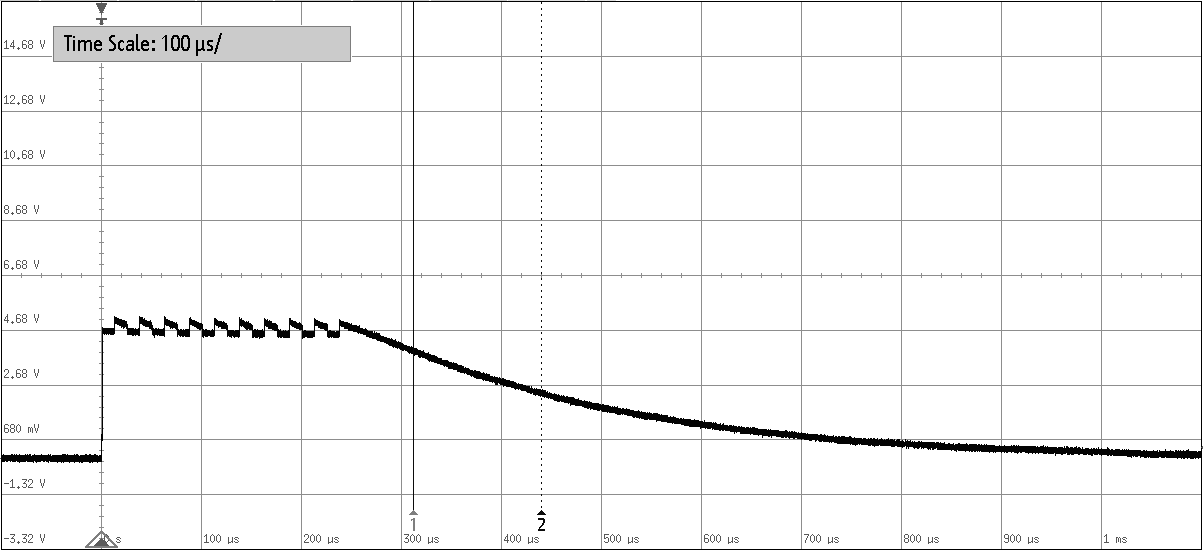
\includegraphics[width=1\textwidth, draft]{Abbildungen/PWM-ausgabe-mit-Hi-Side.png}
\captionof{figure}{PWM Ausgabe über einen Hi-Side}
\label{fig:HiSide}
\end{minipage}

In der Abbildung \ref{fig:pwm-burst} ist zu sehen, dass ein Burst aus zehn Impulsen mit einer Periodendauer von jeweils 25us generiert wurde. Diese Messung wurde direkt an dem Mikrocontroller vorgenommen, um zu überprüfen, wie sich das Signal durch die eingesetzten Bauteile verändert.\\
Die Abbildung \ref{fig:HiSide} zeigt, wie das Ausgangssignal nach der Hi-Side aussieht. So wird zwar im Takt des PWM-Signals geschaltet, allerdichgs fehlt es an einem Gegenpool, um das Potential in den Schaltpausen wieder auf Null zu ziehen. Dadurch bleibt das Signal während des Schaltens immer auf einem erhöhten Pegel und sinkt erst nach Ende des Signals langsam ab. Dadurch kann natürlich keine vernünftige Ausgabe am Lautsprecher erzeugt werden, denn ohne deutliche Potentialunterschiede kann dieser auch nicht richtig schwingen. Der ausgegebene Schalldruck würde maximal für kürzeste Entfernungsmessungen reichen, wenn überhaupt und dann würde das zurückkommende Signal noch von der abklingenden Spannung des Hi-Side überlagert. Dadurch ist dieser Aufbau nicht operabel.\newpage
Wird das Signal über eine Halbbrücke geschaltet, um das Potential auch auf Null ziehen zu können, ergibt sich das folgende Bild. \ref{fig:Halfbridge}.\\
\begin{minipage}{0.5\textwidth}
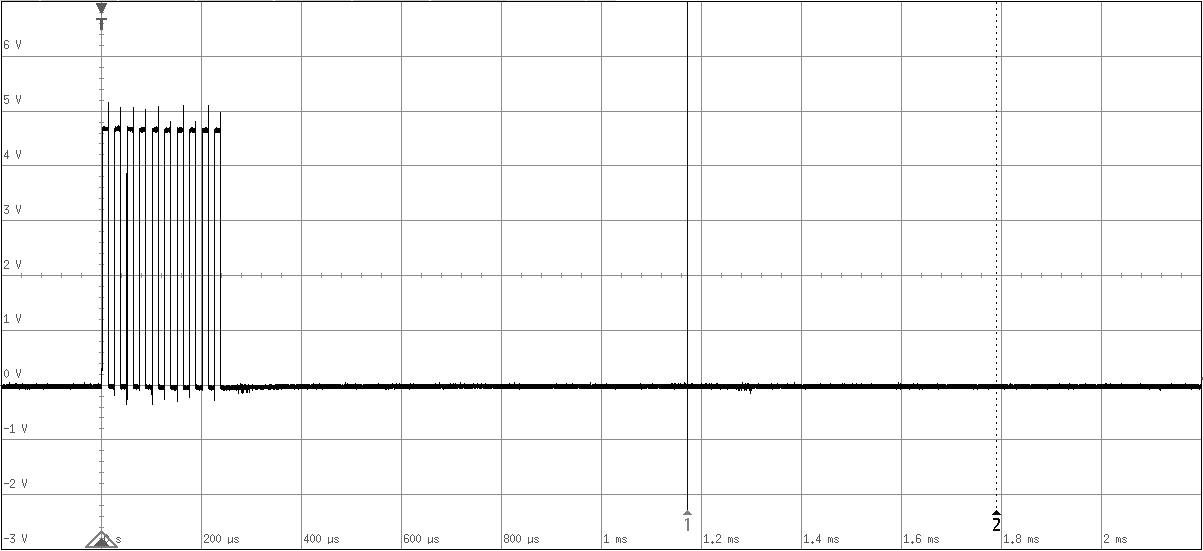
\includegraphics[width=1\textwidth, draft]{Abbildungen/PWM-Nach-der-Halbbrucke.png}
\captionof{figure}{PWM Ausgabe über eine Halbbrucke}
\label{fig:Halfbridge}
\end{minipage}
\begin{minipage}{0.5\textwidth}
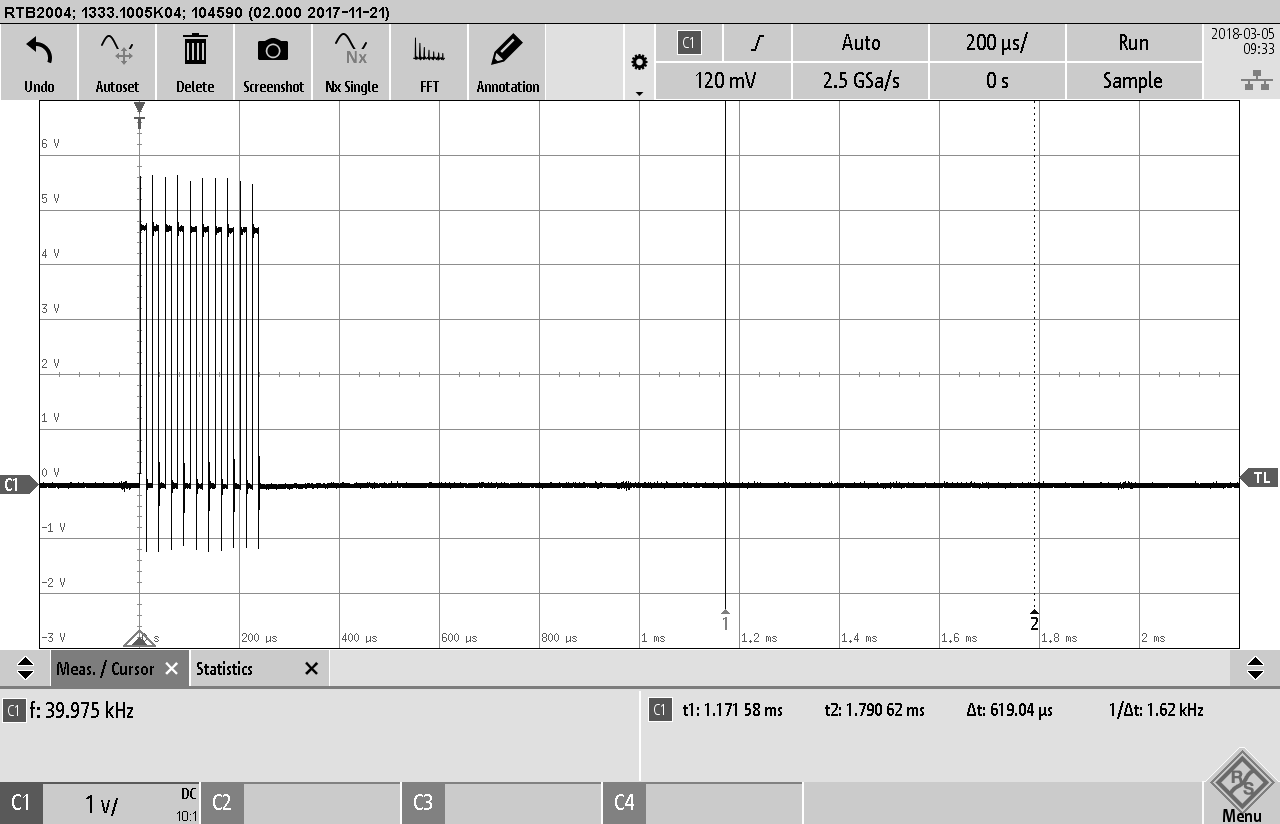
\includegraphics[width=1\textwidth, draft]{Abbildungen/PWM-Nach-der-Halbbrucke-mit-LS.png}
\captionof{figure}{Ausgabe der PWM mit erhöhter Amplitude am Sender}
\label{fig:Sender}
\end{minipage}
Es zeigt sich, dass das Signal nach der Erweiterung auf eine Halbbrücke wieder wie das von der CPU ausgegebene PWM-Signal \ref{fig:pwm-burst} aussieht, nur dass die Amplitude wie geplant höher ausfällt. Somit kann die Höhe der Amplitude über die Spannungspumpe variiert werden um die Stärke des ausgegebenen Signals zu variieren, ohne die CPU durch die höhere Spannung zu beschädigen.
Wie in der Abbildung \ref{fig:Sender} zu entnehmen ist, entstehen durch den angeschlossenen Sender noch Spannungsimpulse im Schaltmoment.

%\section{H-Brücke}
%Mach ersten Versuchen wurde die H-Brücke durch einen IXDN602, einen MOSFET ersetzt. Dies geschah, weil erstens die Beschaltung des OPV nur für eine positive Halbwelle funktioniert und zweitens die Beschaltung der H-Brücke fehlerhaft war. So wurde einer der Ausgänge auf Masse gelegt, was im Betrieb einen Kurzschluss verursachen würde. Um diese Probleme zu beheben, müssten der Sender- und der Empfängerkreis aufgetrennt werden und eine zweite Ultrashallkapsel eingesetzt werden. Dadurch ließ sich eine Reihe an Tests an der Senderschaltung durchführen. Allerdings viel auf, dass im Betrieb keine Signale empfangen wurden. Der Grund dafür war, dass der Mosfet als Low-Side-Driver geschaltet war, was bedeutet dass er das Signal entweder auf High, oder auf Low zieht. Somit werden auch alle von der Ultraschallkapsel empfangenen Signale direkt auf Low gezogen. Also musste eine weitere Überlegung angestellt werden und es wurden aus einem Mosfet zwei. Einer, der vom Prozessor angesteuert wird(3.3V) und den zweiten, der die Sendespannung(5V-20V) freigibt, schaltet. 
\section{Empfangseinheit}
In den ersten Versuchen wurde die Empfangseinheit auf einer zweiten Platine getrennt vom Sender getestet, um eine mögliche Überlagerung der elektrischen Signale zu verhindern. Dafür wurden beide Platinen auf einem Versuchsaufbau befesting und die Sender- und die Empfängerkapsel nebeneinander, parallel ausgerichtet, befestigt.\\
\begin{minipage}{0.5\textwidth}
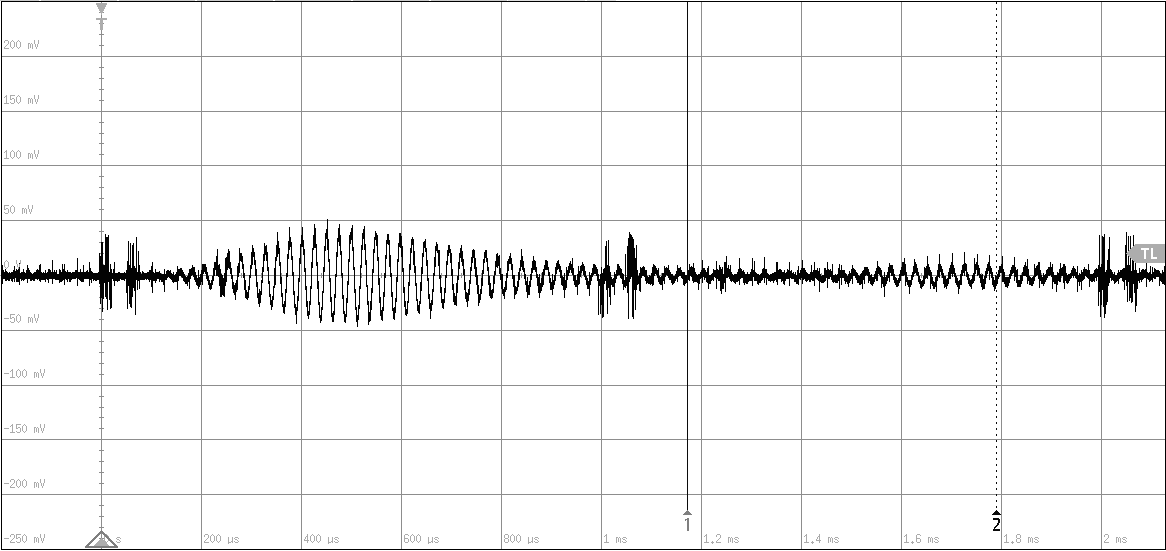
\includegraphics[width=1\textwidth, draft]{Abbildungen/Signal-Empfang.png}
\captionof{figure}{Signal Empfang}
\label{fig:Empfang am LS}
\end{minipage}
\begin{minipage}{0.5\textwidth}
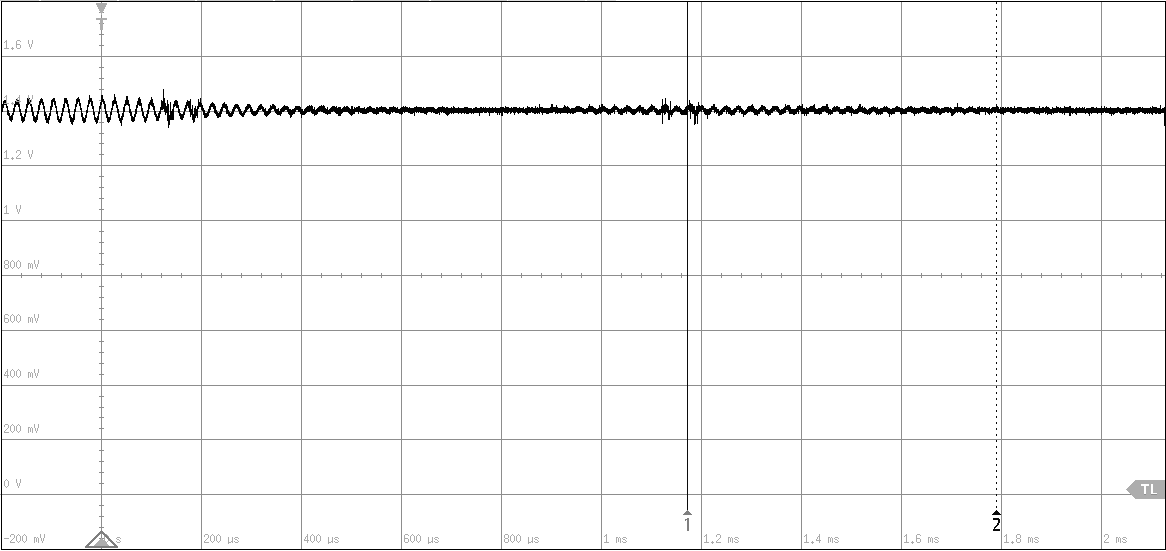
\includegraphics[width=1\textwidth, draft]{Abbildungen/Signal-nach-der-Filterung.png}
\captionof{figure}{Signal nach der Filterung}
\label{fig:Filterung}
\end{minipage}
Die Abbildung \ref{fig:Empfang am LS} zeigt das Signal, das direkt am Empfänger zu messen war. Hier sind verschiedene vorerst nicht zuordnenbare Signale zu sehen. Allein aus diesem Bild lässt sich aber keine Aussage zu den Signalen machen, fest steht nur dass ebenfalls Signale, die nicht der gewünschten Frequenz entsprechen ebenfalls vom Empfänger aufgenommen werden. Diese gilt es natürlich schnellst möglich auszumerzen, um unerwünschte Störungen zu vermeiden.
In der Abbildung \ref{fig:Filterung} ist das Signal nach dem eingebauten Hochpassfilter zu sehen.\\
\begin{minipage}{0.5\textwidth}
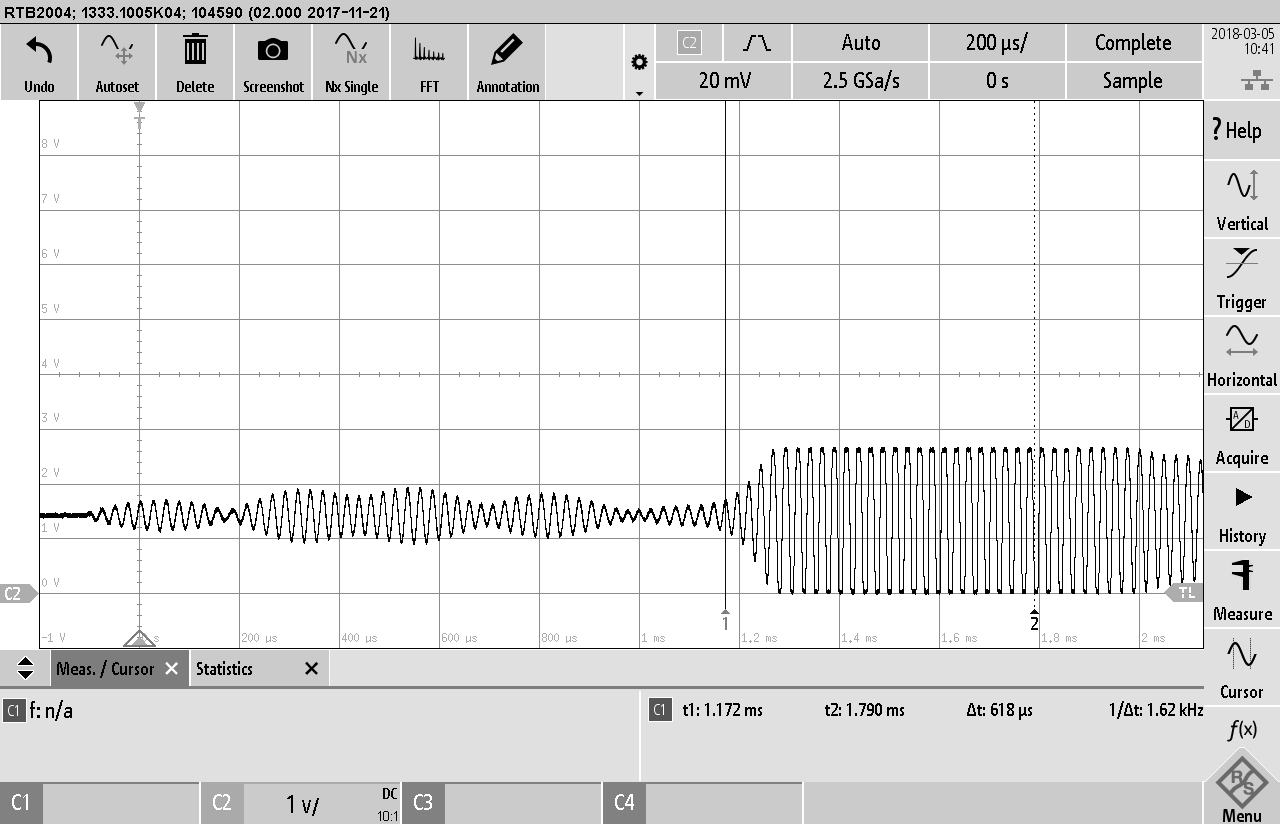
\includegraphics[width=1\textwidth, draft]{Abbildungen/Signal-nach-Verstarkung.png}
\captionof{figure}{Signal nach Verstärkung}
\label{fig:Verstaerkung}
\end{minipage}
\begin{minipage}{0.5\textwidth}
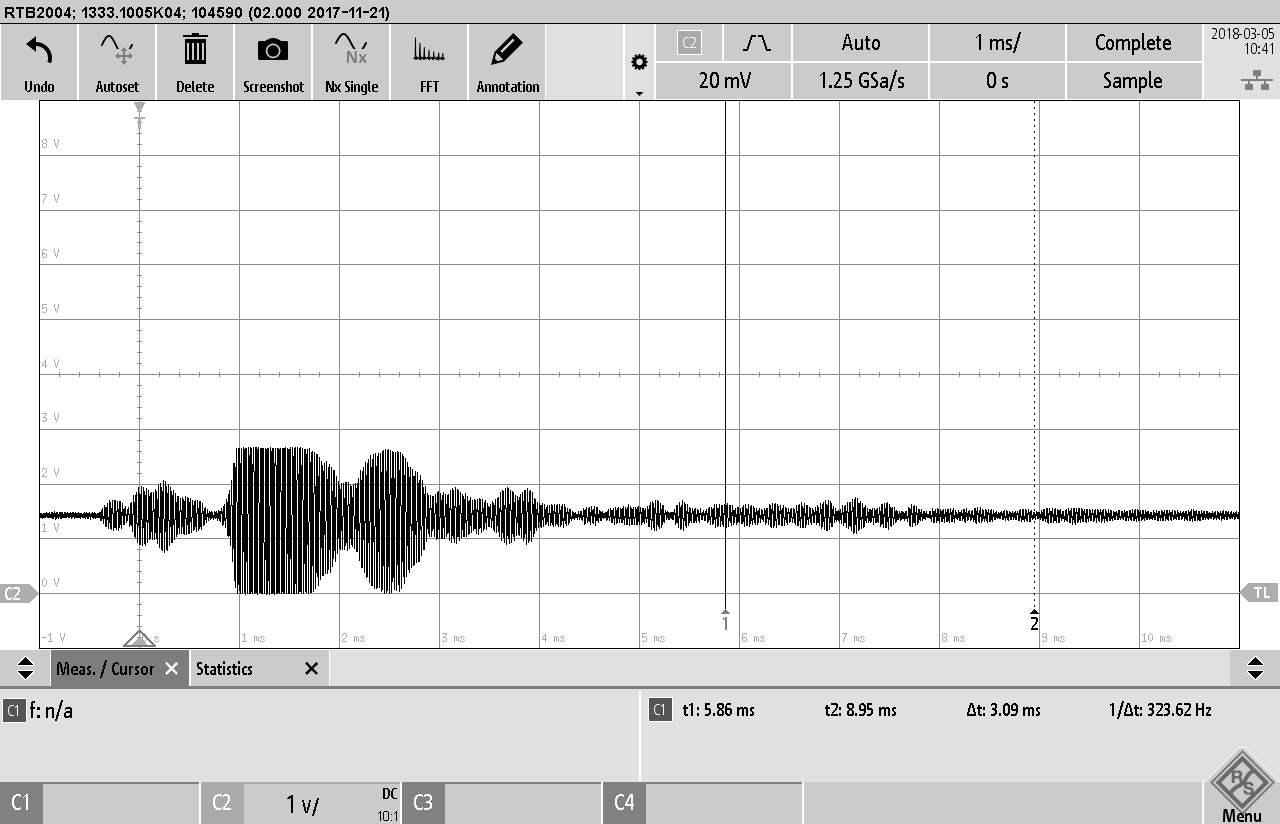
\includegraphics[width=1\textwidth, draft]{Abbildungen/Signal-nach-Verstarkung2.png}
\captionof{figure}{Signal nach Verstärkung2}
\label{fig:Verstaerkung2}
\end{minipage}
Der erste Operationsverstärker dient der Verstärkung des gefilterten Eingangssignals. Dieses ist notwendig, da das ausgesendete Schallsignal mit zunehmendem Weg an Schalldruck verliert, und beim Eintreffen am Empfänger deutlich niedrigere Spannungen erzeugt, als beim absenden eingesetzt wurden. \\
\begin{minipage}{0.6\textwidth}
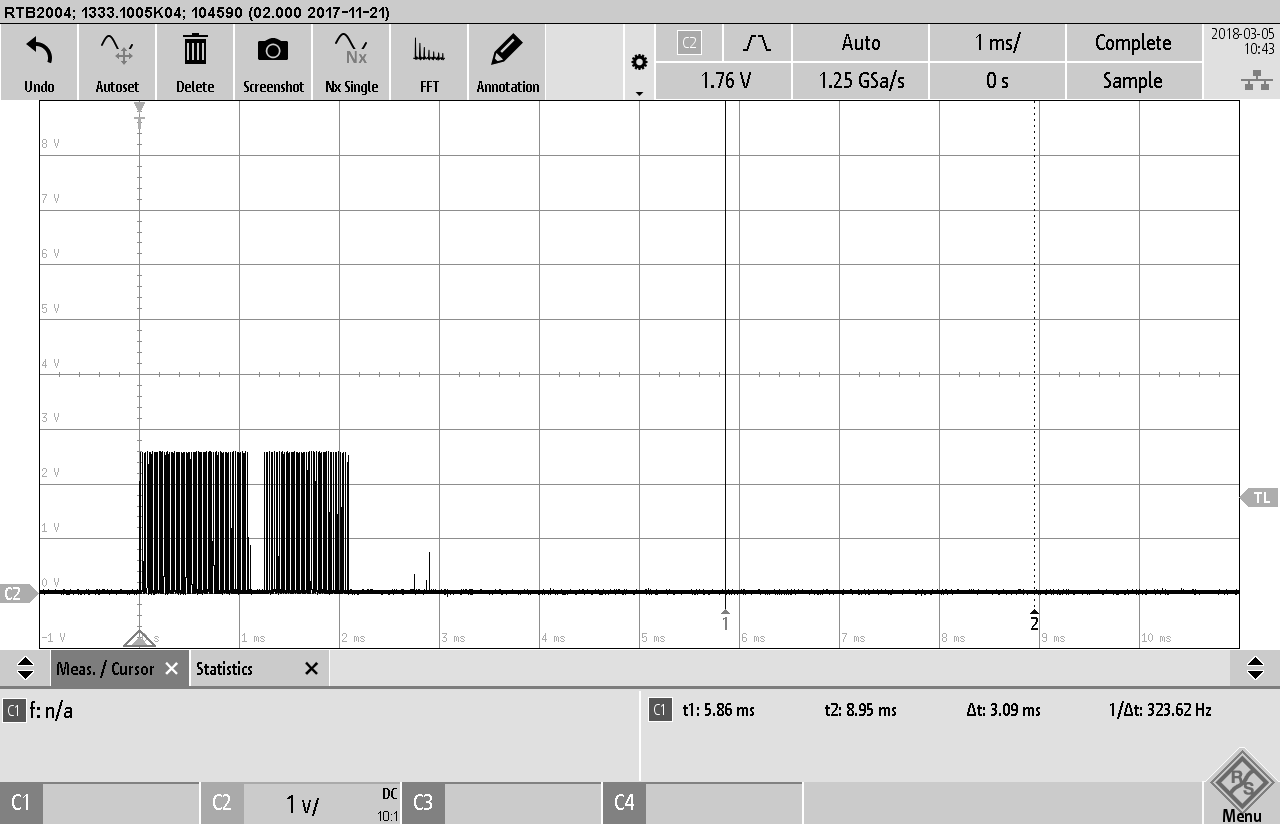
\includegraphics[width=1\textwidth, draft]{Abbildungen/Signal-nach-Komperator.png}\captionof{figure}{Signal nach Komperator}\label{fig:Komperator}
\end{minipage}\\
Nach dem das Signal den Komperator passiert hat, ergibt sich das Bild wie in Abbildung \ref{fig:Komperator} zu sehen ist. Aus dem anfänglichen Eingangssignal, aus dem nichts verwertbares abzulesen war, ist ein wesentlich übersichtligeres Signal entstanden. Nun sind lediglich zwei Signalblöcke übriggeblieben, die beide eine Frequenz von 40kHz haben. Bei dem ersten Signalblock handelt es sich um ein Störsignal, denn es ist das vom Sender ausgesandte Signal, das seitlich auf den Empfänger abstrahlt. Der zweite Signalblock ist dagegen das Echo, also das Signal, das vom Hindernis zurückgeworfen wurde. Mit diesem Signal ließe sich die Entfernung zum Hinderniss berechnen.\\
Nachfolgend wurden die Signalverläufe mit verschiedenen Ultraschallkapseln aufgenommen, um vergleichen zu können, wie die Signalqualität bei verschiedenen Produkten schwankt. Dabei wurde die Amplitude von 4,6V für das Sendersignal nicht verändert.\\
\begin{minipage}{0.5\textwidth}
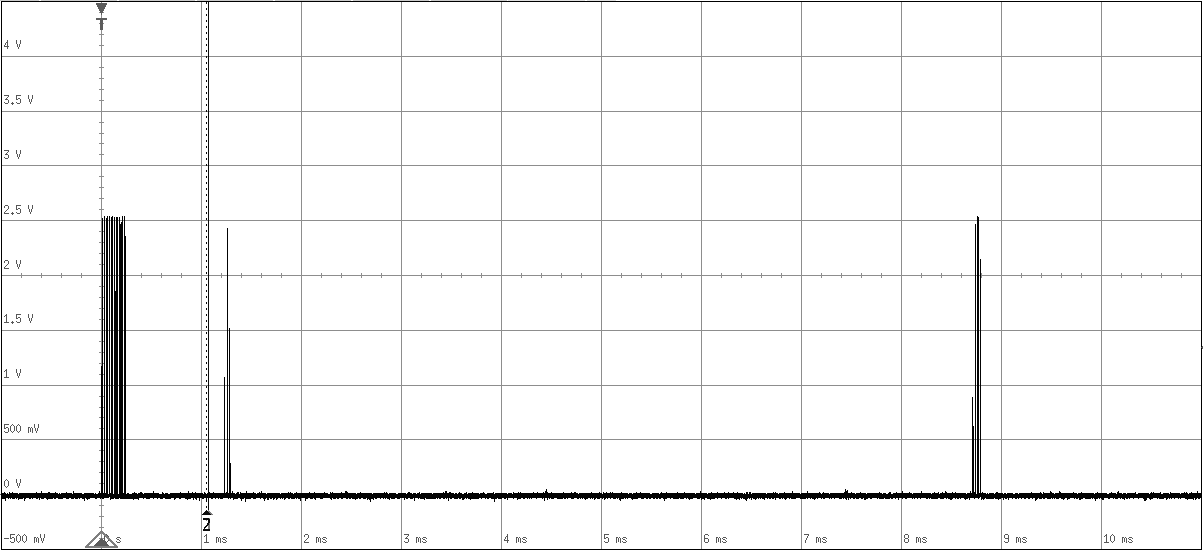
\includegraphics[width=1\textwidth, draft]{Abbildungen/Messungen4,6V/EKULIT1,5m.png}
\captionof{figure}{EKULIT}
\label{fig:EKULIT1,5m}
\end{minipage}
\begin{minipage}{0.5\textwidth}
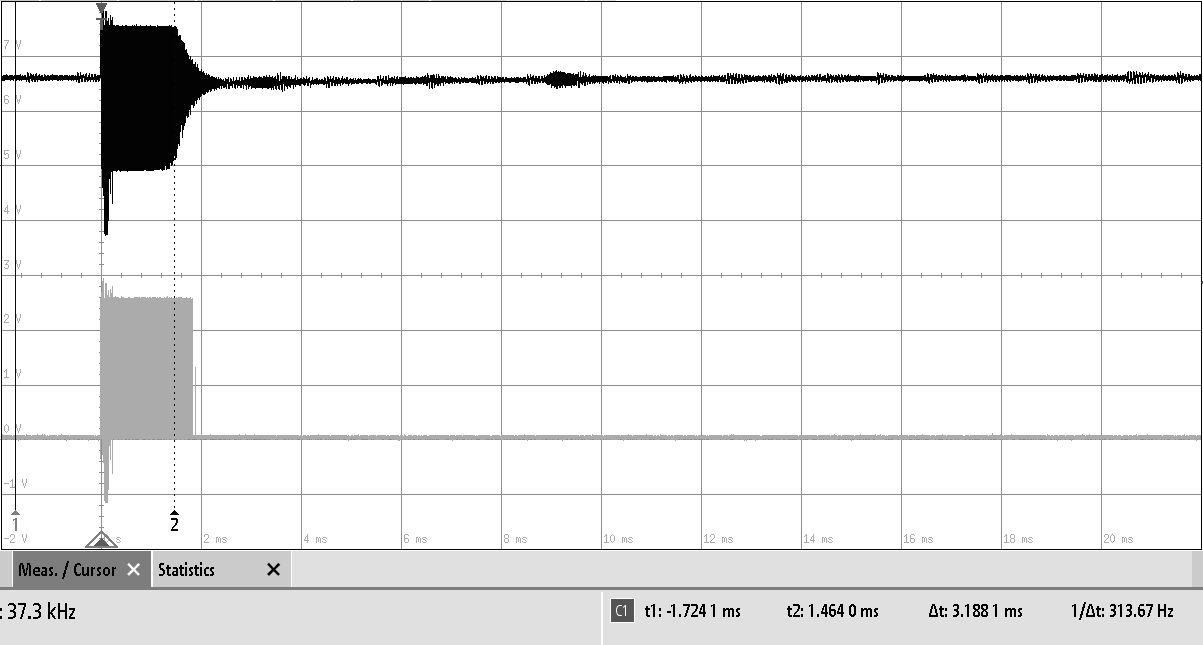
\includegraphics[width=1\textwidth, draft]{Abbildungen/Messungen4,6V/MURATAr1,5m.png}
\captionof{figure}{MURATA reciver}
\label{fig:EKULIT1,5m}
\end{minipage}
\begin{minipage}{0.5\textwidth}
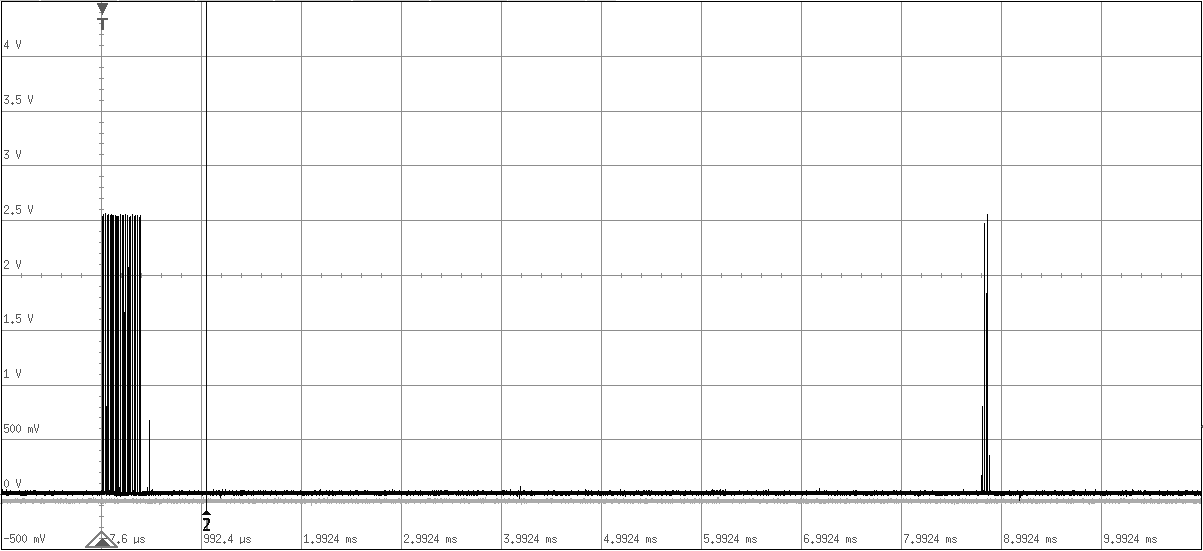
\includegraphics[width=1\textwidth, draft]{Abbildungen/Messungen4,6V/MURATAs1,5m.png}
\captionof{figure}{MURATA sender}
\label{fig:EKULIT1,5m}
\end{minipage}
\begin{minipage}{0.5\textwidth}
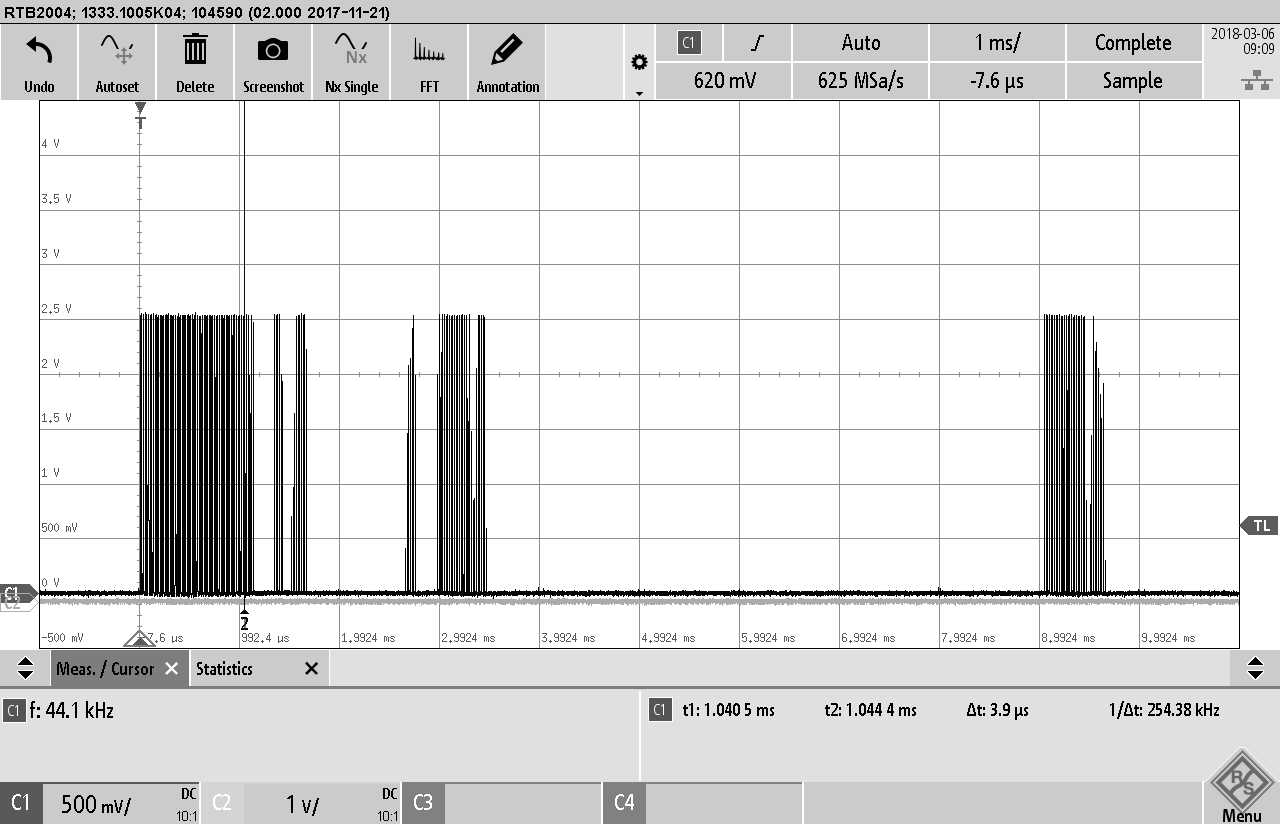
\includegraphics[width=1\textwidth, draft]{Abbildungen/Messungen4,6V/MURATAsr1,5m.png}
\captionof{figure}{MURATA sender+reciver}
\label{fig:EKULIT1,5m}
\end{minipage}


%\section{Signalverlauf nach Verstärkung durch den OPV}
%Durch die Verbindung der Sender- und der Empfängerseite entstand das Problem, dass die Entstörkondensatoren am Empfänger durch den Sendebetrieb zu sehr aufgeladen wurden, und sich danach erstmal entladen mussten, was eine Spannung am Sender/Empfänger zur Folge hatte. Das Entladen der Kondensatoren dauerte länger als die Pausen zwischen den Sendeimpulsen, dadurch konnten keine Signale empfangen werden.Um dieses Problem zu beheben wurde versucht, die OPV's durch einen MOSFET vom Sensor zu trennen, so lange gesendet wird. Da dieses erfolglos blieb wurde der Empfänger durch eine weitere Filterstufe erweitert.
